\documentclass[a4paper,12pt]{article}

\usepackage[margin=2cm]{geometry}
\usepackage{amsmath}
\usepackage{amssymb}
\usepackage{enumitem}
\usepackage{tikz}
\usepackage{pgfplots}

\pgfplotsset{compat=1.18}

\setlength{\parindent}{0pt}
\setlength{\parskip}{0.8em}

\begin{document}

% ============================================================
% Task 1
% ============================================================

\section*{Task 1: Frequency, wavelength and velocity of propagation}

\[
c = f\lambda = \frac{\lambda}{T},
\qquad
c = 343\,\mathrm{m/s}
\]

Calculate the missing quantities:

\begin{center}
\renewcommand{\arraystretch}{1.5}
\begin{tabular}{c|c|c}
$f$ & $\lambda$ & $T$ \\ \hline
$440\,\mathrm{Hz}$ & $0.5\,\mathrm{m}$ & \\[2mm]
$200\,\mathrm{Hz}$ & $1.7\,\mathrm{m}$ & $0.02\,\mathrm{s}$ \\[2mm]
$1000\,\mathrm{Hz}$ & $2\,\mathrm{cm}$ &
\end{tabular}
\end{center}


% ============================================================
% Task 2
% ============================================================

\section*{Task 2: Multiple choice}

\begin{enumerate}[label=$\square$]
    \item A higher frequency means a longer wavelength.
    \item A higher frequency means a shorter wavelength.
    \item Frequency and wavelength are independent of each other.
    \item The speed of sound changes when the frequency changes.
\end{enumerate}


% ============================================================
% Task 3
% ============================================================

\section*{Task 3}

A flute plays a note with a frequency of

\[
f = 523\,\mathrm{Hz}.
\]

Calculate the wavelength of the sound in air. Use

\[
c = 343\,\mathrm{m/s}.
\]


% ============================================================
% Task 4
% ============================================================

\section*{Task 4}

A loudspeaker produces a sound wave with a wavelength of

\[
\lambda = 2\,\mathrm{m}.
\]

Calculate its frequency.


% ============================================================
% Task 5
% ============================================================

\section*{Task 5}

A loudspeaker first plays a tone of $200\,\mathrm{Hz}$ and then a tone of
$600\,\mathrm{Hz}$.

For each quantity, discuss whether it increases, decreases, or stays
the same:

\begin{itemize}
    \item frequency
    \item wavelength
    \item speed of sound
\end{itemize}


% ============================================================
% Task 6
% ============================================================

\section*{Task 6}

Two sound waves travel through air.

\[
\begin{aligned}
\text{Wave A:}\quad &200\,\mathrm{Hz},\\
\text{Wave B:}\quad &800\,\mathrm{Hz}.
\end{aligned}
\]

Discuss:

\begin{itemize}
    \item Which wave has the higher frequency?
    \item Which wave has the longer wavelength?
    \item Which wave travels faster?
\end{itemize}


\newpage

% ============================================================
% Task 7
% ============================================================

\section*{Task 7: Drawing waves}

Consider the following wave.

\begin{center}
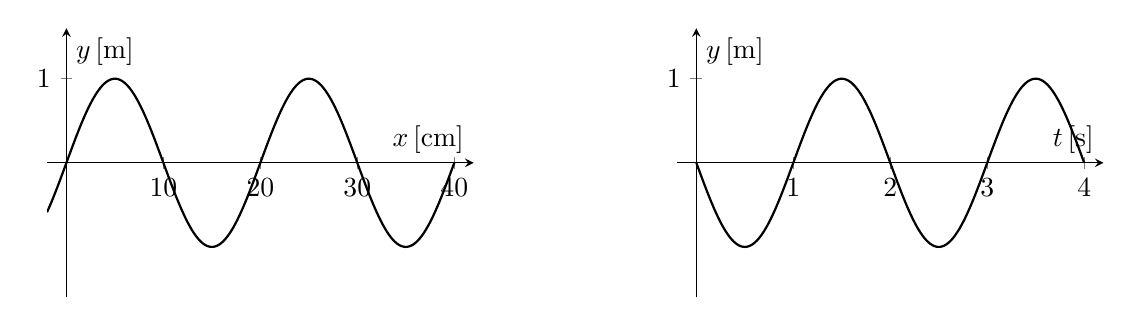
\begin{tikzpicture}[>=stealth]

% --- spatial wave ---
\begin{axis}[
    width=7cm,
    height=5cm,
    axis lines=middle,
    xlabel={$x\, [\mathrm{cm}]$},
    ylabel={$y\, [\mathrm{m}]$},
    xmin=-2, xmax=42,
    ymin=-1.6, ymax=1.6,
    xtick={10,20,30,40},
    ytick={1},
    samples=200,
    domain=-2:40,
    axis line style={->},
]
\addplot[thick]
    {sin(deg(2*pi*x/20))};
\end{axis}

% --- time wave ---
\begin{axis}[
    at={(8cm,0cm)},
    width=7cm,
    height=5cm,
    axis lines=middle,
    xlabel={$t\, [\mathrm{s}]$},
    ylabel={$y\, [\mathrm{m}]$},
    xmin=-0.2, xmax=4.2,
    ymin=-1.6, ymax=1.6,
    xtick={1,2,3,4},
    ytick={1},
    samples=200,
    domain=0:4,
    axis line style={->},
]
\addplot[thick]
    {-sin(deg(pi*x))};
\end{axis}

\end{tikzpicture}
\end{center}

Discuss:

\begin{itemize}
    \item Which graph shows the motion of one oscillator?
    \item Which graph shows the shape of the entire wave at one instant?
    \item What is shown on the horizontal axis of each graph?
    \item From which graph can you determine the period $T$?
    \item From which graph can you determine the wavelength $\lambda$?
    \item Determine $c$, $\lambda$, $f$, and $T$.
\end{itemize}


\subsection*{What changes if the amplitude is doubled?}

Draw the changes.

\begin{center}
\begin{tikzpicture}[>=stealth]

% spatial graph
\begin{axis}[
    width=7cm,
    height=4.5cm,
    axis lines=middle,
    xlabel={$x\, [\mathrm{cm}]$},
    ylabel={$y\, [\mathrm{m}]$},
    xmin=-2, xmax=42,
    ymin=-2.5, ymax=2.5,
    xtick={10,20,30,40},
    ytick={1},
    axis line style={->},
]
\end{axis}

% temporal graph
\begin{axis}[
    at={(8cm,0cm)},
    width=7cm,
    height=4.5cm,
    axis lines=middle,
    xlabel={$t\, [\mathrm{s}]$},
    ylabel={$y\, [\mathrm{m}]$},
    xmin=-0.2, xmax=4.2,
    ymin=-2.5, ymax=2.5,
    xtick={1,2,3,4},
    ytick={1},
    axis line style={->},
]
\end{axis}

\end{tikzpicture}
\end{center}


\subsection*{What happens if $c$ stays constant and $f$ is increased by a factor of 2?}

Draw the changes.

\begin{center}
\begin{tikzpicture}[>=stealth]

% spatial graph
\begin{axis}[
    width=7cm,
    height=4.5cm,
    axis lines=middle,
    xlabel={$x\, [\mathrm{cm}]$},
    ylabel={$y\, [\mathrm{m}]$},
    xmin=-2, xmax=42,
    ymin=-1.6, ymax=1.6,
    xtick={10,20,30,40},
    ytick={1},
    axis line style={->},
]
\end{axis}

% temporal graph
\begin{axis}[
    at={(8cm,0cm)},
    width=7cm,
    height=4.5cm,
    axis lines=middle,
    xlabel={$t\, [\mathrm{s}]$},
    ylabel={$y\, [\mathrm{m}]$},
    xmin=-0.2, xmax=4.2,
    ymin=-1.6, ymax=1.6,
    xtick={1,2,3,4},
    ytick={1},
    axis line style={->},
]
\end{axis}

\end{tikzpicture}
\end{center}


\newpage

% ============================================================
% Harmonic waves
% ============================================================

\section*{Harmonic Waves}

Read the following statements about a harmonic wave.
Decide whether the statements are \textbf{True} or \textbf{False}.

\begin{enumerate}[label=$\square$]
    \item Every point oscillates harmonically.
    \item The wave transports matter from one place to another.
    \item Every point oscillates with the same frequency.
    \item Neighbouring points have a phase difference.
    \item Every point has the same amplitude.
\end{enumerate}

If a statement is false, discuss why.


\vspace{1cm}

Discuss the similarities and differences between travelling harmonic
and standing waves.


\newpage

% ============================================================
% Standing waves
% ============================================================

\section*{Standing Waves}

Draw the standing wave pattern for:

\begin{itemize}
    \item the fundamental mode,
    \item the first overtone,
    \item the second overtone.
\end{itemize}

Mark all nodes and antinodes.

Distinguish between two fixed ends, one fixed and one free end,
and two free ends.

\subsection*{Two fixed ends}

\begin{center}
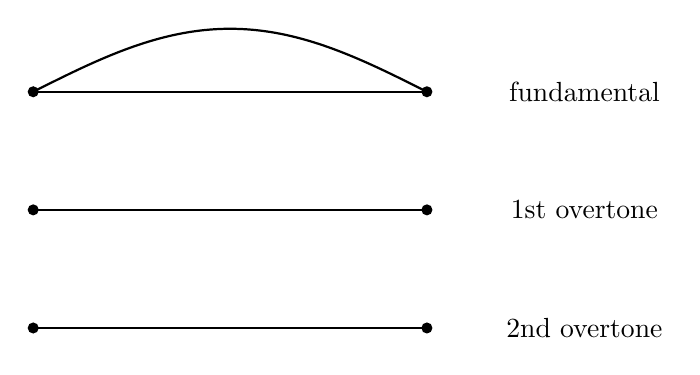
\begin{tikzpicture}

% Fundamental
\draw[thick] (0,0) -- (5,0);
\fill (0,0) circle (2pt);
\fill (5,0) circle (2pt);

\draw[thick] plot[domain=0:5,samples=100]
    (\x,{0.8*sin(180*\x/5)});

\node at (7,0) {fundamental};

% First overtone
\begin{scope}[yshift=-1.5cm]
\draw[thick] (0,0) -- (5,0);
\fill (0,0) circle (2pt);
\fill (5,0) circle (2pt);

\node at (7,0) {1st overtone};
\end{scope}

% Second overtone
\begin{scope}[yshift=-3cm]
\draw[thick] (0,0) -- (5,0);
\fill (0,0) circle (2pt);
\fill (5,0) circle (2pt);

\node at (7,0) {2nd overtone};
\end{scope}

\end{tikzpicture}
\end{center}


\subsection*{One fixed end and one free end}

\begin{center}
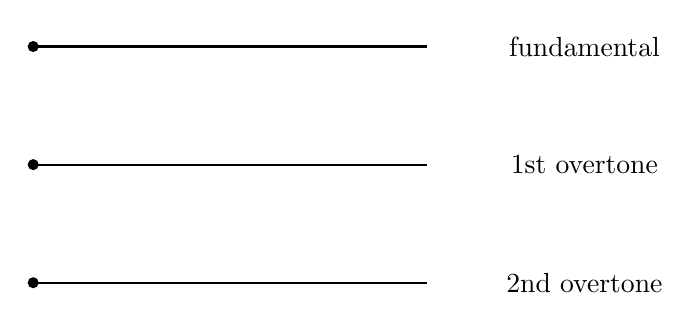
\begin{tikzpicture}

\draw[thick] (0,0) -- (5,0);
\fill (0,0) circle (2pt);
\node at (7,0) {fundamental};

\begin{scope}[yshift=-1.5cm]
\draw[thick] (0,0) -- (5,0);
\fill (0,0) circle (2pt);
\node at (7,0) {1st overtone};
\end{scope}


\begin{scope}[yshift=-3cm]

\draw[thick] (0,0) -- (5,0);
\fill (0,0) circle (2pt);

\node at (7,0) {2nd overtone};
\end{scope}

\end{tikzpicture}
\end{center}


\subsection*{Two open ends}

\begin{center}
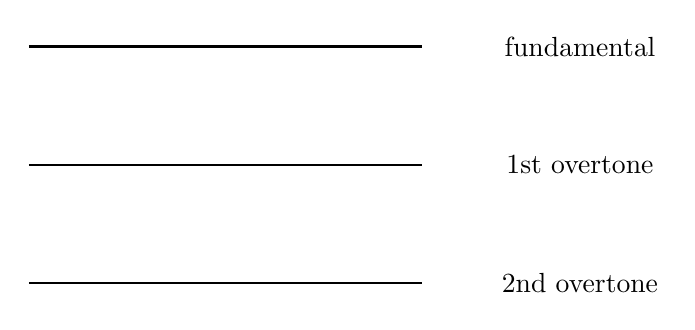
\begin{tikzpicture}

\draw[thick] (0,0) -- (5,0);
\node at (7,0) {fundamental};

\begin{scope}[yshift=-1.5cm]
\draw[thick] (0,0) -- (5,0);
\node at (7,0) {1st overtone};
\end{scope}

\begin{scope}[yshift=-3cm]
\draw[thick] (0,0) -- (5,0);
\node at (7,0) {2nd overtone};
\end{scope}

\end{tikzpicture}
\end{center}


\subsection*{Nodes and antinodes}

How are nodes and antinodes distributed?

What is the distance between two nodes / antinodes?


\vspace{1cm}

Consider a string with the length

\[
L = 1.2\,\mathrm{m}
\]

which is fixed at both ends.

Calculate the wavelength of:

\begin{itemize}
    \item the fundamental mode,
    \item the first overtone,
    \item the second overtone.
\end{itemize}

\end{document}